
\documentclass[12pt]{article}
\usepackage[english,finnish]{babel}
\usepackage{t1enc}

% AMS packages:
\usepackage{amsbsy}
\usepackage{amsfonts}
\usepackage{amsmath}
\usepackage{amssymb}
\usepackage{amsthm}
\usepackage{amsxtra}
% for comments to work
\usepackage{verbatim}
\usepackage{hyperref}
\usepackage{graphicx}
\usepackage{bbold}
\usepackage{bbm}
\usepackage{float}

%%%%%%%%%%%%%%%%%%%%%%%%%%%%%%%%%%%

% Hilbert spaces:
\newcommand{\hilb}{\mathcal{H}}
\newcommand{\banH}{\mathcal{B}(\hilb)}
\newcommand{\fock}{\mathcal{F}}

% Products:
\newcommand{\scalpr}[2]{( #1, #2 )}
\newcommand{\dualpr}[2]{\langle #1, #2 \rangle}

% Fonts
\newcommand{\calc}{\mathcal{C}}
\newcommand{\cala}{\mathcal{A}}
\newcommand{\calv}{\mathcal{V}}
\newcommand{\calf}{\mathcal{F}}
\newcommand{\cals}{\mathcal{S}}
\newcommand{\cald}{\mathcal{D}}
\newcommand{\banach}{\mathcal{B}}
\newcommand{\id}[1]{\mathbbm{1}\!\left({#1}\right)}

\newcommand{\ci}{{\rm i}}
\newcommand{\rmd}{{\rm d}}
\newcommand{\rme}{{\rm e}}

\newcommand{\re}{{\rm Re\,}}
\newcommand{\im}{{\rm Im\,}}

% misc
\newcommand{\defem}[1]{{\em #1\/}}
\newcommand{\vep}{\varepsilon}


\newcommand{\qand}{\quad\text{and}\quad}

% To define sets:
\newcommand{\defset}[2]{ \left\{ #1 \left|\, #2\makebox[0pt]{$\displaystyle\phantom{#1}$}\right.\!\right\} }

\newcounter{alplisti}
\renewcommand{\thealplisti}{\alph{alplisti}}
\newenvironment{alplist}[1][(\thealplisti)]{\begin{list}{{\rm #1}\ }{ %
      \usecounter{alplisti} %
    \setlength{\itemsep}{0pt}
    \setlength{\parsep}{0pt}  %
     \setlength{\topsep}{0pt} %
}}{\end{list}}

% Norms:
\newcommand{\abs}[1] {\lvert #1 \rvert}
\newcommand{\norm}[1]{\lVert #1 \rVert}
\newcommand{\floor}[1] {\lfloor {#1} \rfloor}
\newcommand{\ceil}[1]  {\lceil  {#1} \rceil}

% Basic spaces
\newcommand{\R} {\mathbb{R}}
\newcommand{\C} {{\mathbb{C}}}
\newcommand{\Rd} {{\mathbb{R}^{d}}}
\newcommand{\N} {\mathbb{N}}
\newcommand{\Z} {\mathbb{Z}}
\newcommand{\Q} {\mathbb{Q}}
\newcommand{\K} {\mathbb{K}}
\newcommand{\T} {\mathbb{T}}

%%%%%%%%%%%%%%%%%%%%%%%%%%%%%%%%%%%


\newcommand{\pat}{\partial}
\newcommand{\be}{\begin{equation}}
\newcommand{\ee}{\end{equation}}
\newcommand{\bea}{\begin{eqnarray}}
\newcommand{\eea}{\end{eqnarray}}
\newcommand{\abf}{{\bf a}}
\newcommand{\Zcal}{{\cal Z}_{12}}
\newcommand{\zcal}{z_{12}}
\newcommand{\Acal}{{\cal A}}
\newcommand{\Fcal}{{\cal F}}
\newcommand{\Ucal}{{\cal U}}
\newcommand{\Vcal}{{\cal V}}
\newcommand{\Ocal}{{\cal O}}
\newcommand{\Rcal}{{\cal R}}
\newcommand{\Scal}{{\cal S}}
\newcommand{\Lcal}{{\cal L}}
\newcommand{\Hcal}{{\cal H}}
\newcommand{\hsf}{{\sf h}}
\newcommand{\half}{\frac{1}{2}}
\newcommand{\Xbar}{\bar{X}}
\newcommand{\xibar}{\bar{\xi }}
\newcommand{\barh}{\bar{h}}
\newcommand{\Ubar}{\bar{\cal U}}
\newcommand{\Vbar}{\bar{\cal V}}
\newcommand{\Fbar}{\bar{F}}
\newcommand{\zbar}{\bar{z}}
\newcommand{\wbar}{\bar{w}}
\newcommand{\zbarhat}{\hat{\bar{z}}}
\newcommand{\wbarhat}{\hat{\bar{w}}}
\newcommand{\wbartilde}{\tilde{\bar{w}}}
\newcommand{\barone}{\bar{1}}
\newcommand{\bartwo}{\bar{2}}
\newcommand{\nbyn}{N \times N}
\newcommand{\repres}{\leftrightarrow}
\newcommand{\Tr}{{\rm Tr}}
\newcommand{\tr}{{\rm tr}}
\newcommand{\ninfty}{N \rightarrow \infty}
\newcommand{\unitk}{{\bf 1}_k}
\newcommand{\unitm}{{\bf 1}}
\newcommand{\zerom}{{\bf 0}}
\newcommand{\unittwo}{{\bf 1}_2}
\newcommand{\holo}{{\cal U}}
\newcommand{\bra}{\langle}
\newcommand{\ket}{\rangle}
\newcommand{\muhat}{\hat{\mu}}
\newcommand{\nuhat}{\hat{\nu}}
\newcommand{\rhat}{\hat{r}}
\newcommand{\phat}{\hat{\phi}}
\newcommand{\that}{\hat{t}}
\newcommand{\shat}{\hat{s}}
\newcommand{\zhat}{\hat{z}}
\newcommand{\what}{\hat{w}}
\newcommand{\sgamma}{\sqrt{\gamma}}
\newcommand{\bfE}{{\bf E}}
\newcommand{\bfB}{{\bf B}}
\newcommand{\bfM}{{\bf M}}
\newcommand{\cl} {\cal l}
\newcommand{\ctilde}{\tilde{\chi}}
\newcommand{\ttilde}{\tilde{t}}
\newcommand{\ptilde}{\tilde{\phi}}
\newcommand{\utilde}{\tilde{u}}
\newcommand{\vtilde}{\tilde{v}}
\newcommand{\wtilde}{\tilde{w}}
\newcommand{\ztilde}{\tilde{z}}

\newcommand{\Mob}{\text{Mob}}


\selectlanguage{english}

\hoffset 0.5cm
\voffset -0.4cm
\evensidemargin -0.2in
\oddsidemargin -0.2in
\topmargin -0.2in
\textwidth 6.3in
\textheight 8.4in

\begin{document}

\normalsize

\baselineskip 14pt

\begin{center}
{\Large {\bf FYMM/MMP IIIa 2020 \ \ \  Solutions to Problem Set 4}}
\\
Jake Muff
24/9/20
\end{center}

\bigskip



\begin{enumerate}
\item Question 1
$$ D_4 = \langle r,f | r^4 ,f^2, rfrf \rangle $$
Where $r = 90 \text{ degree rotation}$ and $f = $ reflection. Need to find and motivate the presentation for $D_n$. Clearly $r^4 = e$ as this is equivalent to a 360 degree rotation and clearly $f^2 = e $ due to it being reflected twice. $rfrf = e$ as well. 
\\
For a polygon with $n$ sides it can be rotated by 360 degree as the operation r and reflected by f. The $n$ sided polygon will always naturally have 2 reflections, one after the other to return it to its original state due to a natural property of reflections so for $D_n$ $f^2 = e$ always. 
\\
The $n$ sided polygon rotated $n$ times through through rotation $r$ will also similarly return it to its original state as a nature of the rotation around a point, therefore $r^n = e $. 
\\
Also a reflection ($f$) then a rotation ($r$) then a reflection ($f$) then a rotation ($r$) where $r$ is 90 degrees will always be the identity for $n$ sided polygons. So
$$ D_n = \langle r,f | r^n, f^2, rfrf \rangle $$ 
\item Draw a picture of the braid (of 4 strands) $\sigma_3\sigma^{-1}_1\sigma^{-1}_2\sigma_3\sigma_1\sigma_3$.
\\
\begin{figure}[h]
  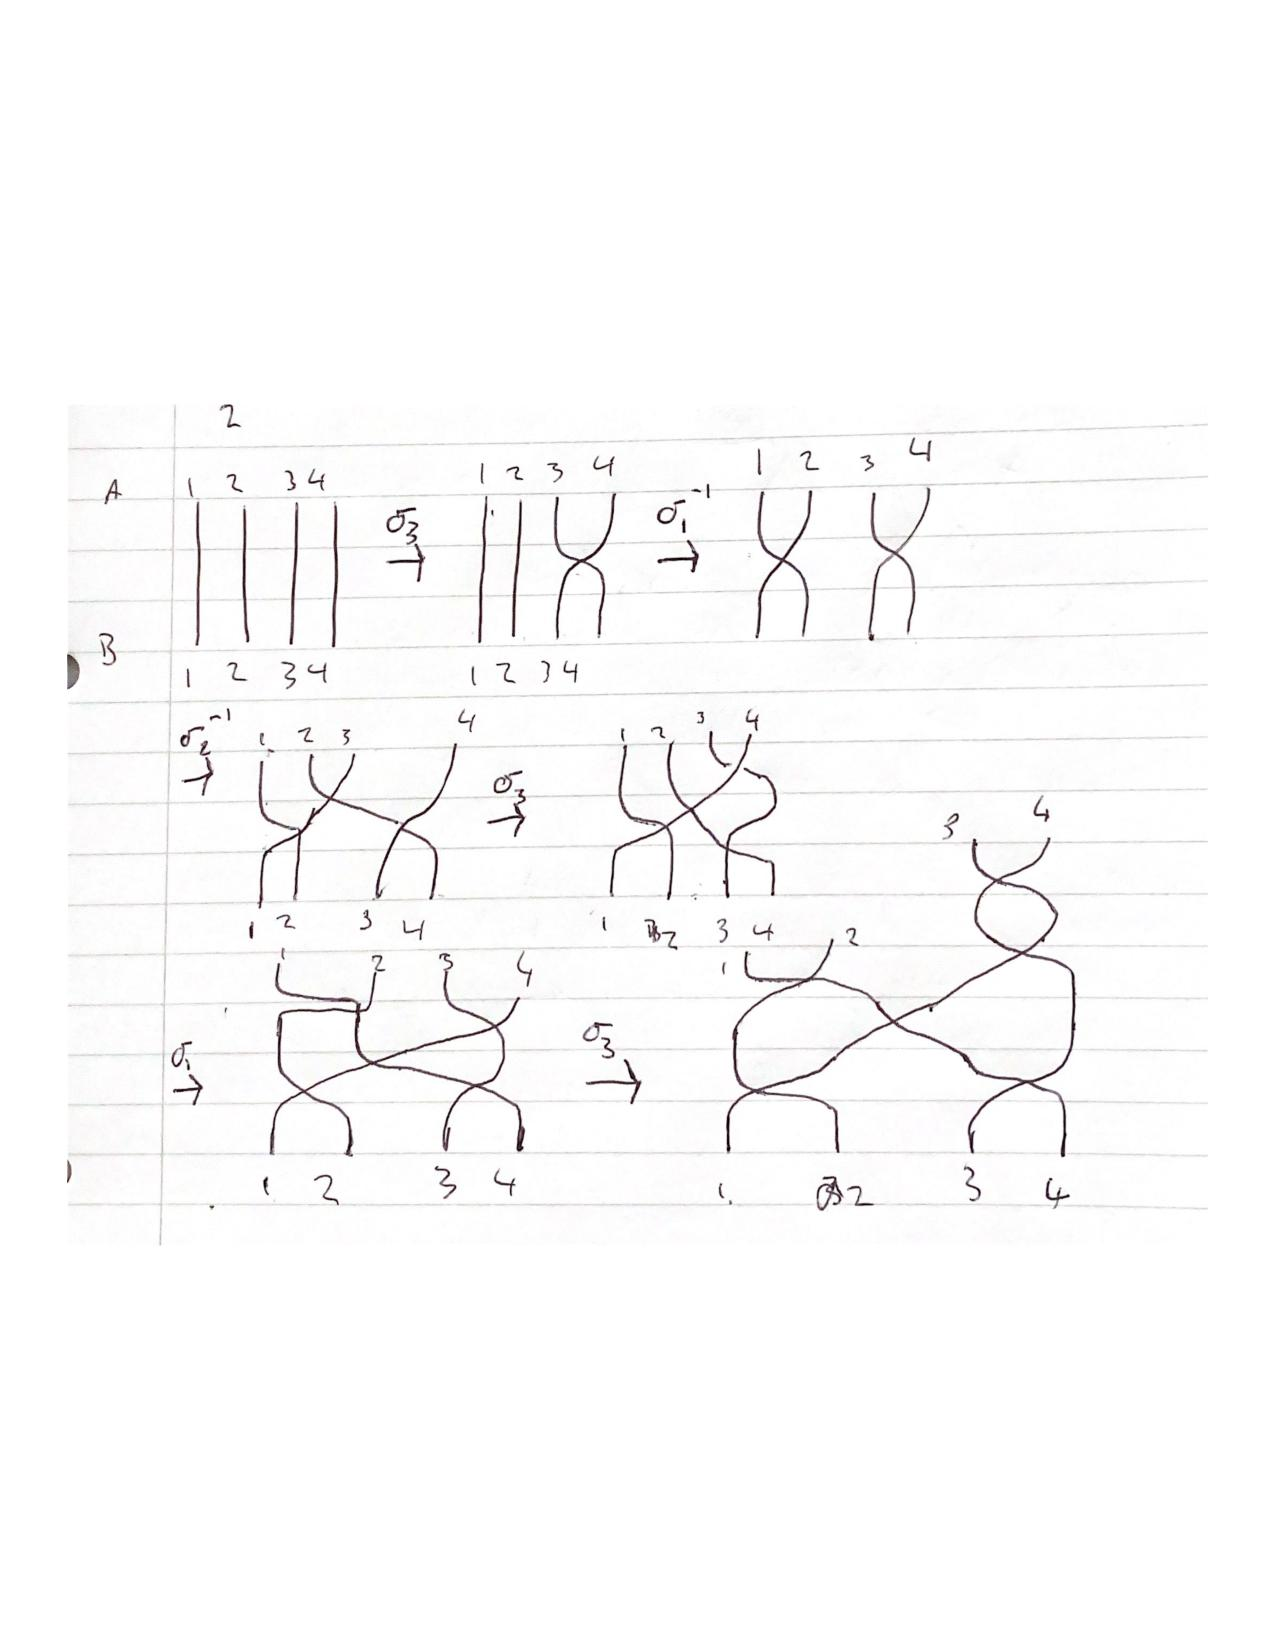
\includegraphics[width=10cm]{Braids.jpg}
  \centering 
  \caption{Process of me creating the braid going through each step}

\end{figure}
$\sigma_i^{-1}$ moves the $i+1$ strand over the $i$th strand. $\sigma_3$ moves the 3rd strand over the 4th strand. $\sigma_1^{-1}$ moves the 2nd strand over the first strand. $\sigma_2^{-1}$ moves the 3rd strand over the 2nd strand. $\sigma_1$ moves the 1st strand over the 2nd strand and $\sigma_3$ moves the 3rd strand over the 4th strand. When drawing we take the equation from left to right and draw from the bottom up. 
\begin{figure}[H]
  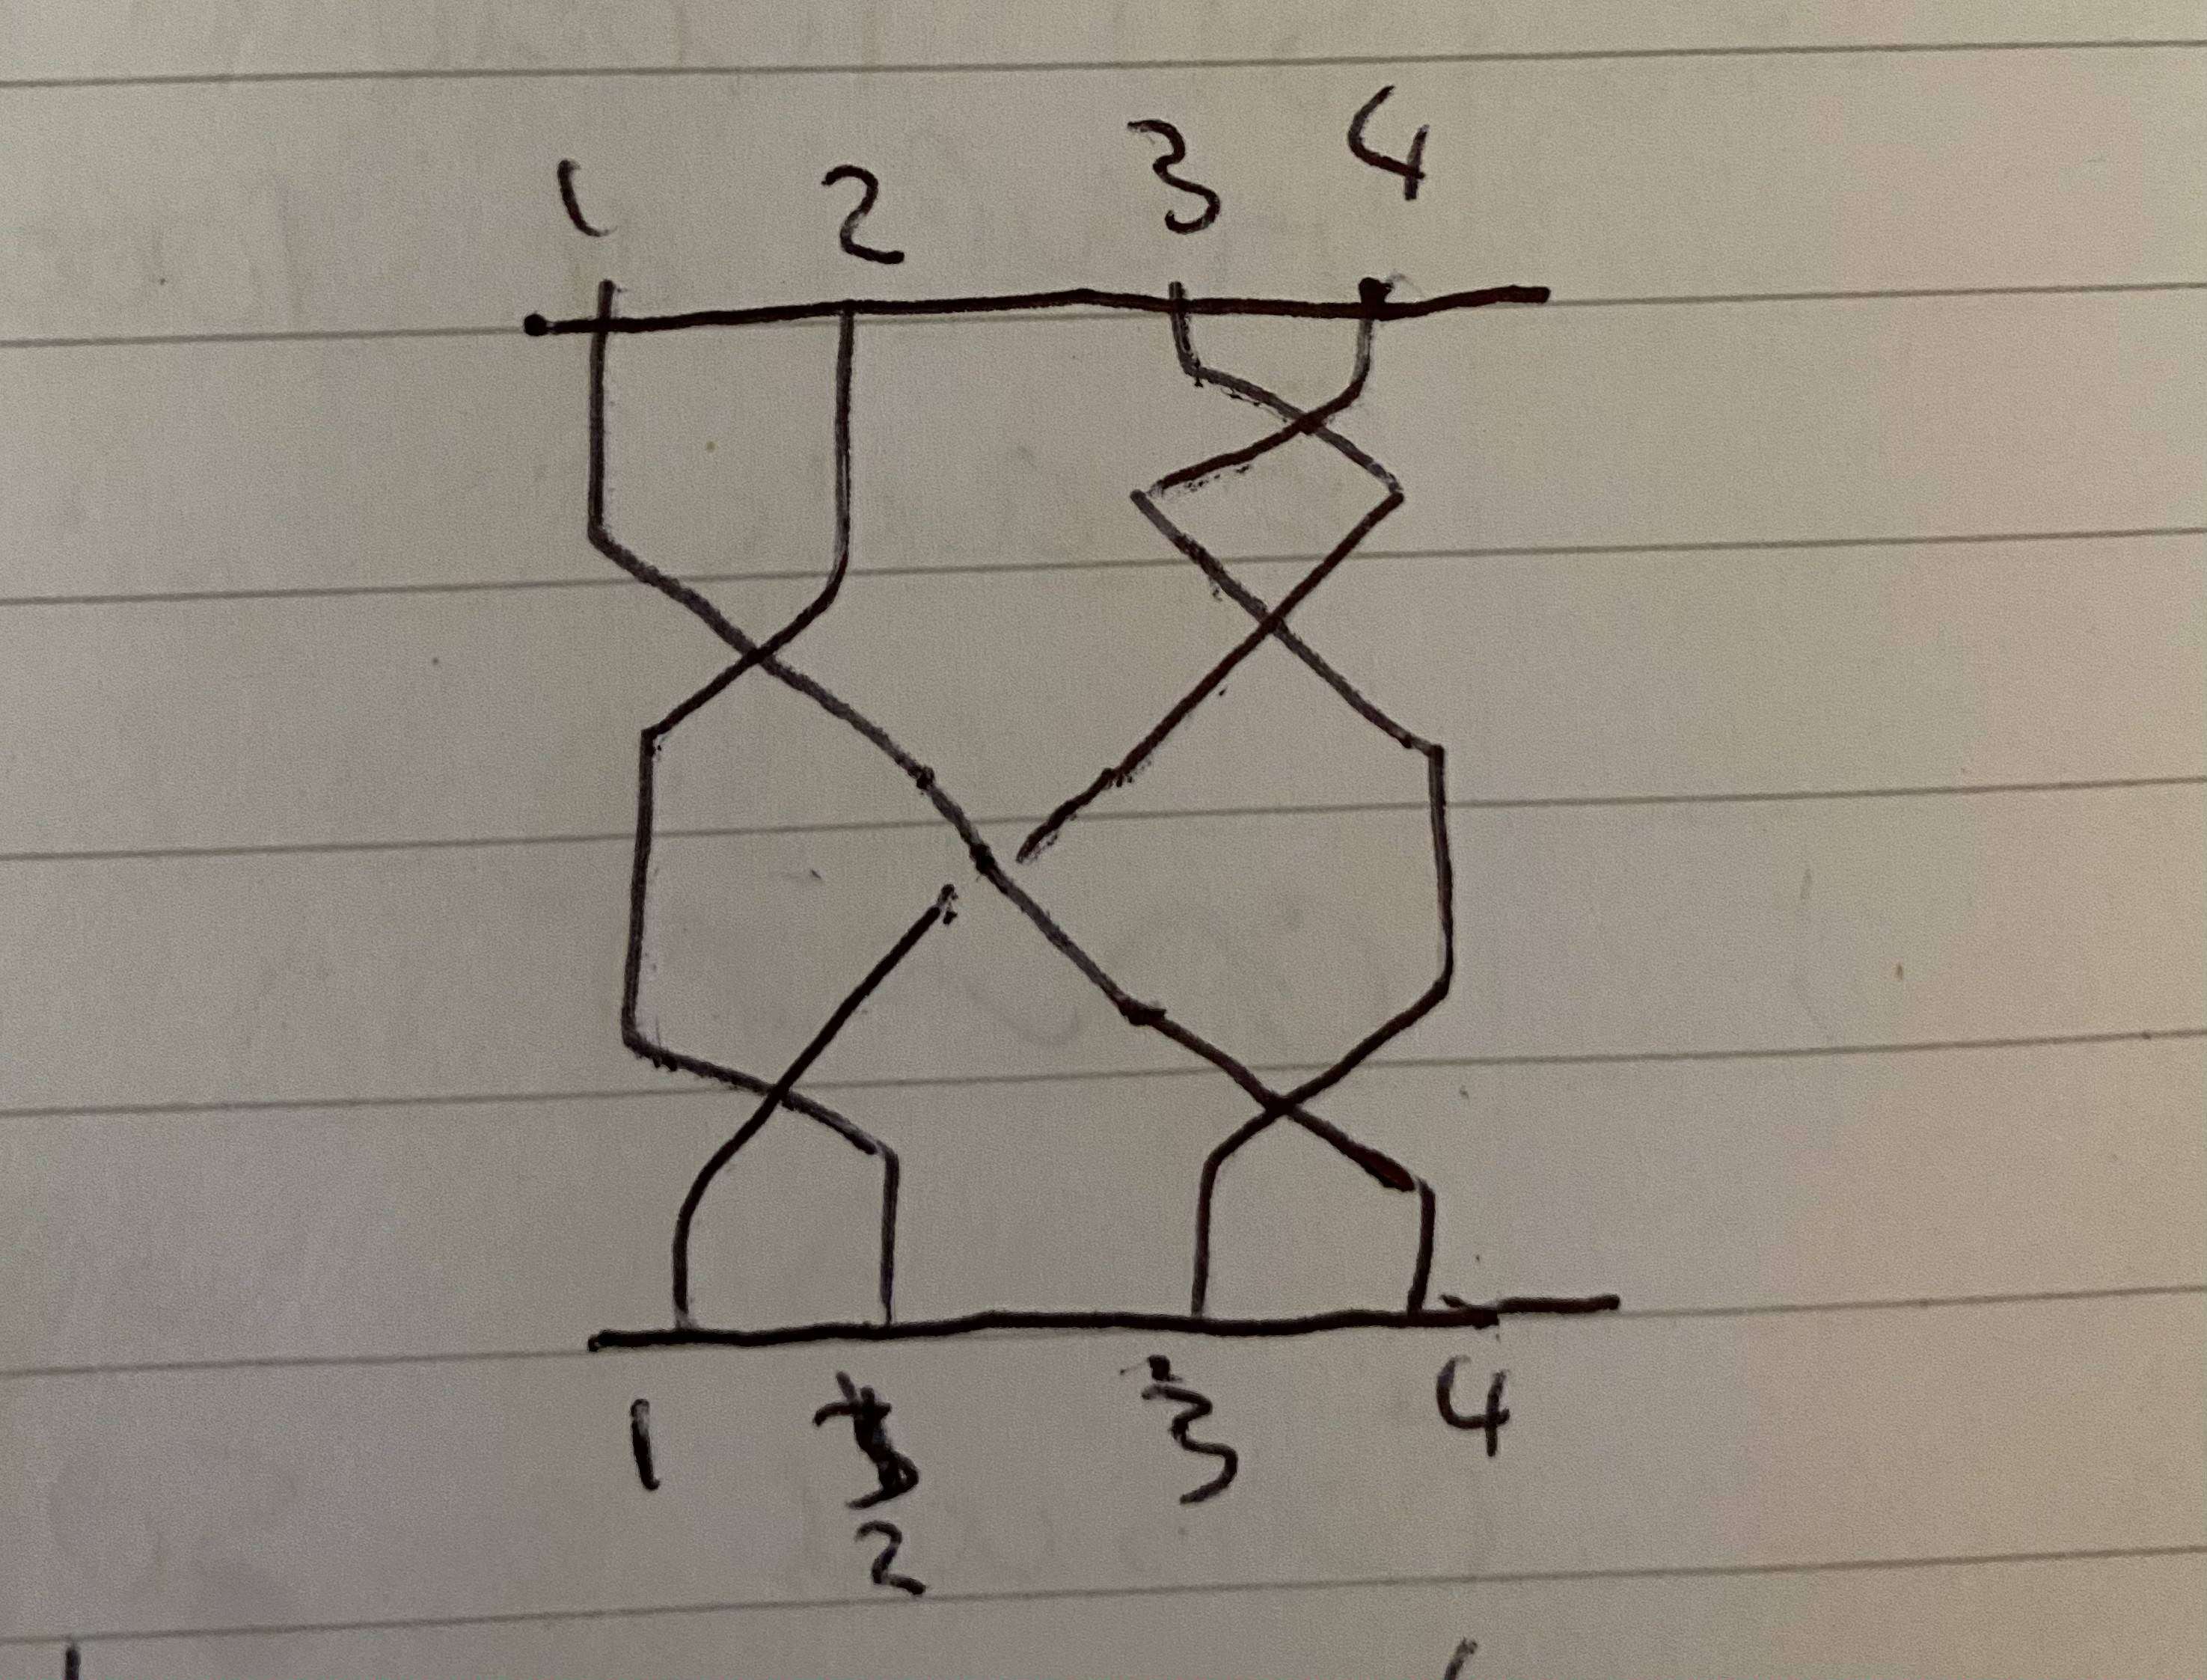
\includegraphics[width=10cm]{answer.jpg}
  \centering 
  \caption{Drawing of the braid in final form}

\end{figure}
\pagebreak
\item Question 3
\\
SO(3) left action on the sphere $S^2 \in \Re^3$. SO(3) is the 3D rotation group i.e the group of rotations of the xy plane about the z axis. 
\\
Didn't really understand how to use the vector $x$ to parametrize this isotropy group. 
\item Consider the set of {\em M\"obius transformations}
\begin{equation}
\Mob  = \left\{f_A:\mathbb{C}\to\mathbb{C}|f_A(z) = \frac{az+b}{cz+d};\,A=\left(\begin{array}{cc} a&b\\ c&d  \end{array} \right)\in SL(2,\mathbb{C})  \right\}
\end{equation}
\begin{enumerate}
\item Show that $\Mob $ is a group, with composition of mappings as the product.
\\
To show this go through the usual steps to prove a group, starting with closure and associativity (G0 \& G1). \\
Let $f_A, f_B \in \Mob$ with $SL$ matrices 
$$ \left(\begin{array}{cc} a&b\\ c&d  \end{array} \right) \ ; \left(\begin{array}{cc} a'&b'\\ c'&d'  \end{array} \right)$$
Such that 
$$ (f_B \circ f_A ) (z) = \frac{a'a + b'c)z + (b'b+b'd)z}{(c'a + cd')z + (cd' + dd')z} $$
$$ = f_{BA} (z)$$
With $BA$ the product of $B$ and $A$, $BA \in SL$ and $f_{BA} \in \Mob$. Proving closure with associativity inherited. \\
For G2, the exitence of the unit element. The unit element of \Mob is $f_{\mathbb{1}}$ which is the complex identity $f_{\mathbb{1}} = id_c$ so we have
$$ f_A \circ f_{\mathbb{1}} = f_{A\mathbb{1}} = f_A = f_{\mathbb{1}} \circ f_A $$
Now we know trivially that $\mathbb{1} \in SL$ amd $f_{\mathbb{1}} \in \Mob$. \\
Existence of the inverse. 
$$ A^{-1} \in SL $$
$$ f_A \circ f_{A^{-1}} = f_{AA^{-1}} = f_{\mathbb{1}} = f_{A^{-1}} \circ f_A $$
So 
$$ f_{A^{-1}} = f_A^{-1} $$ 
And it is a group. 

\item Show that the mapping
\begin{equation}
f: SL(2,\mathbb{C})\to \Mob ;\,f(A)=f_A
\end{equation}
is a homomorphism.\\
For it to be a homomorphism it needs to have $ \forall g_1, g_2 \in G, f(g_1 g_2) = f(g_1)f(g_2)$. So from closure we have 
$$ f(AB) = f_AB = f_A \circ f_B = f(A) \circ f(B) $$ 
So there exists a group homomorphism. 
\item Find a subgroup $H$ of SL$(2,\mathbb{C})$  such that the quotient group SL$(2,\mathbb{C})$/$H$ is isomorphic to $\Mob $. Give reasons why.
\\
Taken inspiration from example at the top of page 22 of the lecture notes. Let $G$ and $H$ be groups such that 
$$ \phi : G \rightarrow H \ \ \text{Be a homomorphism} $$
Then we have 
\begin{enumerate}
  \item Kernel of $\phi$ is a normal subgroup of G 
  \item Image of $\phi$ is a subgroup of H 
  \item Image of $\phi$ is isomorphic to the quotient group $G/Ker(\phi)$ 
\end{enumerate}
The kernel is 
$$ ker(f) = \{ A \in SL(2,\mathbb{C}) | f_A = e = f_{\mathbb{1}} = id_c\} $$
If we expand the condition that 
$$ f_A (z) = z \ \forall z$$
Then we see that $az+b$ is equal to $cz^2 + dz$ where, due to linear independence, $c=b$ and $b=0$ and $a=d$. Now we also have a property that $A \in SL(2, \mathbb{C}) \rightarrow det(A) = 1$ 
Therefore, $a = d = \pm 1$ and the kernel is 
$$ ker(f) = \{ A \in SL(2, \mathbb{C}) | \mathbb{1},\mathbb{-1}\} $$
From the theorem above, part iii, and using part (b) of this question we have 
$$ f: SL(2,\mathbb{C}) \rightarrow \Mob \ ; \ f(A) = f_A $$ 
is a group homomorphism so 
$$ \Mob \cong SL(2,\mathbb{C}) / \mathbb{Z}_2 $$
\end{enumerate}
\item Let $V_1,V_2$ be vector spaces, $L: V_1\rightarrow V_2$ a linear map. Show that $Im L$ and $Ker L$ are vector subspaces of $V_1$ and $V_2$.
\\
%To show that the set is in a subspace, we need to show that for any constant $a$, if $\vec{u}$ and $\vec{v}$ are in the image then so is $a \vec{u} + \vec{v}$. For any $\vec{u}$ and $\vec{v}$ where $\vec{u} = f(x)$ and $\vec{v} = f(y)$ then 
%$$ a \vec{u} + \vec{v} = 
$V_1, V_2$ are vector spaces over a field denoted $F$ \\
The kernel and image of $L$ is 
$$ ker(L) = \{ \vec{v_1} \in V_1 | L(\vec{v_1}) = 0 \} $$
$$ Im(L) = \{ \vec{v_2}\in V_2 | \exists \vec{v_2} \in V_1 s.t L(\vec{v_1})= \vec{v_2}\}$$
To be a vector subspace we need to have that 
$$ u,v \in V \ \text{and} \ u+v \in V$$ 
And
$$ v \in V, u \in V, vu \in V $$
where $u,v$ are vectors and $V$ a vector space and I've replaced the arrow notation. \\
So, for the image $Im(L)$  $u,v \in Im(L)$ there exists a 
$$ w,y \in V_1 \rightarrow L(w) = u \ ; \ L(y) = v$$
$$ u + v = L(w) + L(y) = L(w+y)$$
Hence 
$$ u + v \in Im(L) $$
And for our second condition $u \in Im(L)$ so that $u = L(w)$ for some $w \in V_1$ and a constant $c$ in the field $F$ so that 
$$ cw \in V_1 $$
For all $c \in F$. Then 
$$ cv = c L(w) = L(cw) \in Im(L) $$ 
So Im(L) is a vector subspace. \\
For the kernel we have $u,v \in Ker(L)$ so $L(u) =0$ and $L(v) =0$. Using the same process as before 
$$ L(u + v) = L(u) + L(v) = 0 + 0 = 0 $$ 
So, $u + v \in Ker(L) $. For the second condition we have $u \in ker(L)$ and $c \in F$ so that 
$$ L(c u) = cL(u) = c \cdot 0 =0 $$
So $c u \in Ker(L) $ \\
And $Ker(L)$ is a vector subspace. 

\end{enumerate}

\end{document}
%%%%%%%%%%%%%%%%%%%%%%%%%%
$